%%%%%%%%%%%%%%%%%%%%%%%%%%%%%%%%%
%
%       RESPOSTA QUESTÃO DISCURSIVA
%
%%%%%%%%%%%%%%%%%%%%%%%%%%%%%%%%%
\begin{center}
    \large{\textbf{Resposta da questão discursiva}}
\end{center}
\vspace{20pt}
    
\textbf{Exercício 6}. Vamos escrever a função \(S(t)\) como uma função definida por sentenças. Para isso, note que 
%
\[
    \begin{array}{ccc}
        |t-2| = \left\{
        \begin{array}{rl}
            t - 2, & \text{se } t \ge 2, \\
            -t + 2 & \text{se } t \le 2,
        \end{array}
        \right.
        & \quad \text{ e } \qquad\qquad &
        |t-7| = \left\{
        \begin{array}{rl}
            t - 7, & \text{se } t \ge 7, \\
            -t + 7 & \text{se } t \le 7.
        \end{array}
        \right.
    \end{array}
\]
%
Assim, considerando o diagrama abaixo
%
\begin{center}
    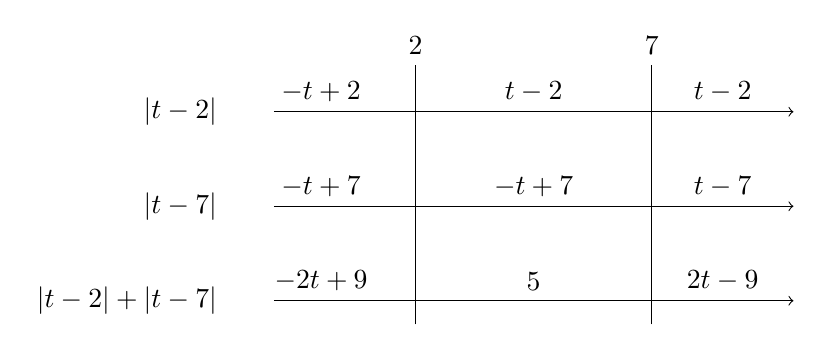
\begin{tikzpicture}[scale=0.6]
        \draw[->] (-1,4) -- (10,4);
        \node[left] at (-2,4) {\(|t-2|\)};
        \node[above] at (0,4) {\(-t+2\)};
        \node[above] at (4.5,4) {\(t-2\)};
        \node[above] at (8.5,4) {\(t-2\)};
        
        \draw[->] (-1,2) -- (10,2);
        \node[left] at (-2,2) {\(|t-7|\)};
        \node[above] at (0,2) {\(-t+7\)};
        \node[above] at (4.5,2) {\(-t+7\)};
        \node[above] at (8.5,2) {\(t-7\)};
        
        \draw[->] (-1,0) -- (10,0);
        \node[left] at (-2,0) {\(|t-2|+|t-7|\)};
        \node[above] at (0,0) {\(-2t+9\)};
        \node[above] at (4.5,0) {\(5\)};
        \node[above] at (8.5,0) {\(2t-9\)};

        \draw[-] (2,-0.5) -- (2,5);
        \draw[-] (7,-0.5) -- (7,5);

        \node[above] at (2,5) {\(2\)};
        \node[above] at (7,5) {\(7\)};
    \end{tikzpicture}
\end{center}
%
obtemos que 
%
\[
    S(t) = |t-2|+|t-7| = \left\{
    \begin{array}{rl}
        -2t + 9, & \text{se } t < 2, \\
        5, & \text{se } 2 \le t < 7, \\
        2t - 9 & \text{se } t \ge 7.
    \end{array}
    \right.
\]
%
Agora, observe que se \(t<2\), então \(S(t) = -2t + 9\) é uma função decrescente cujo mínimo está limitado por \(S(2) = 5\). Se \(t \ge 7\), temos que \(S(t) = 2t + 9\) é uma função crescente cujo mínimo está limitado por \(S(7) = 5\). Como \(S(t) = 5\), para \(2 \le t < 7\), então o valor mínimo de \(S(t)\) é exatamente igual a \(5\). Abaixo, segue o gráfico da função.
\begin{center}
    \begin{tikzpicture}[scale=0.5]
        % Eixos
        \draw[->] (-1,0) -- (9,0) node[right] {\(x\)};
        \draw[->] (0,-.5) -- (0,7) node[above] {\(y\)};

        % Gráfico da função f(x) = |x-2| + |x+3|
        \draw[domain=1:2, thick, blue] plot (\x, {-2*\x +9}); % x < -1
        \draw[domain=2:7, thick, blue] plot (\x, {5});    % x ≥ -1
        \draw[domain=7:8, thick, blue] plot (\x, {2*\x -9});    % x ≥ -1

        % Marcação do vértice (x = -1)
        \draw[dashed] (2,0) -- (2,5);
        \node[below] at (2,0) {\small\(2\)};
        \draw[dashed] (7,0) -- (7,5);
        \node[below] at (7,0) {\small\(7\)};
        \draw[dashed] (0,5) -- (2,5);
        \node[left] at (0,5) {\small\(5\)};
    \end{tikzpicture}
\end{center}
